\documentclass{article}
\usepackage[T1]{fontenc}
\usepackage[utf8]{inputenc}
\usepackage[english, icelandic]{babel}
\usepackage{amsmath}
\usepackage{amssymb}
\usepackage{amsthm}
\usepackage{gensymb}
\usepackage{parskip}
\usepackage{mathtools}
\usepackage{xfrac}
\usepackage{graphicx}
\usepackage{xcolor}
\usepackage{tikz}
\usetikzlibrary{calc}
\usepackage{verbatim}
\usepackage{minted}
\usepackage{multicol}
\parskip 0pt

\DeclareMathOperator{\lcm}{lcm}
\DeclareMathOperator{\diam}{diam}
\DeclareMathOperator{\dist}{dist}
\DeclareMathOperator{\ord}{ord}
\DeclareMathOperator{\Aut}{Aut}
\DeclareMathOperator{\Inn}{Inn}
\DeclareMathOperator{\Ker}{Ker}
\DeclareMathOperator{\trace}{trace}
\DeclareMathOperator{\fix}{fix}
\newcommand\floor[1]{\left\lfloor#1\right\rfloor}
\newcommand\ceil[1]{\left\lceil#1\right\rceil}
\newcommand\abs[1]{\left|#1\right|}
\newcommand\p[1]{\left(#1\right)}
\newcommand\sqp[1]{\left[#1\right]}
\newcommand\cp[1]{\left\{#1\right\}}
\newcommand\norm[1]{\left\lVert#1\right\rVert}
\renewcommand\qedsymbol{$\blacksquare$}

\pagenumbering{gobble}

\graphicspath{{myndir/}}

\begin{document}

\begin{titlepage}
	\centering
	{\scshape\LARGE Háskóli Íslands \par}
	\vspace{1cm}
	{\scshape\Large Töluleg greining \par}
	\vspace{1.5cm}
	{\huge\bfseries Stórt verkefni I \par}
	\vspace{2cm}
	{\Large\itshape Atli Fannar Franklín \\ Hjörvar Logi Ingvarsson\par}
	\vfill
	Kennari: \par
	Sigurður Freyr Hafstein \par 

	\vfill

	{\large \today\par}
\end{titlepage}

Öll hjálparföll sem vitnuð eru í eru gefin aftast í viðauka með öllum hjálparföllum. Í þessu verkefni notuðumst við við sage sem forritunarmálið okkar. Sage er útvíkkun á python, í raun bara python með fullt af pökkum fyrifram (numpy, scipy, sympy, etc.). Fyrst er beðið um að forrita fall $f$ sem tekur inn $\theta$ (liður 1). Þetta fall fá finna í viðaukanum. Ef við prófum fallið á umbeðni inntaki fæst eftirfarandi niðurstaða: \\

\begin{minted}{sage}
sage: x1, x2, y2 = 4, 0, 4
sage: L1, L2, L3 = 2, sqrt(2), sqrt(2)
sage: gam, p1, p2, p3 = pi/2, sqrt(5), sqrt(5), sqrt(5)
sage: f(pi/4)
0.000000000000000
sage: f(-pi/4)
0.000000000000000
\end{minted}

\vspace*{0.5cm}

Nú má teikna graf af $f$ með allar breytur fastar nema $\theta$ með því að nota $g$ hjálparfallið í viðaukanum og skipunina: \\

\begin{small}
\begin{minted}{sage}
sage: h = g(4, 0, 4, 2, sqrt(2), sqrt(2), pi/2, sqrt(5), sqrt(5), sqrt(5))
sage: plot(h, (-pi,pi))
\end{minted}
\end{small}

\vspace*{0.5cm}

Þetta gefur myndina: \\

\begin{center}
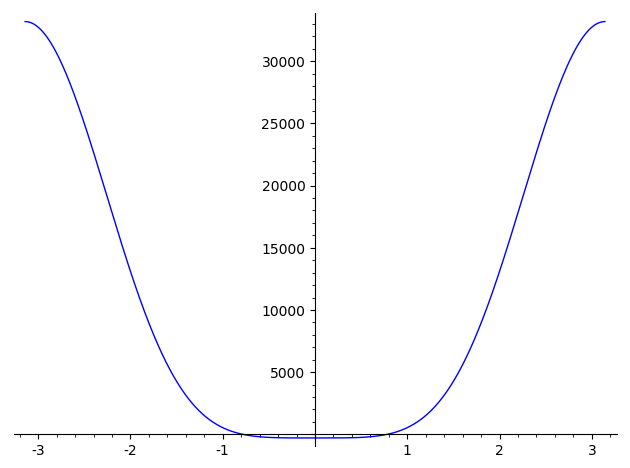
\includegraphics[scale=0.75]{lidur2plot}
\end{center}

\vspace*{0.5cm}

Nú getum við nýtt okkur \verb|plotter| hjálparfallið í viðauka til að teikna myndirnar 15a og 15b í bók upp á nýtt með skipununum: \\

\begin{minted}{sage}
sage: plotter(4, 0, 4, 2, sqrt(2), sqrt(2), 2, 1, pi/4, pi/2)
sage: plotter(4, 0, 4, 2, sqrt(2), sqrt(2), 1, 2, -pi/4, pi/2)
\end{minted}

\vspace*{0.5cm}

Þetta gefur myndirnar: \\

\begin{multicols}{2}
\begin{center}
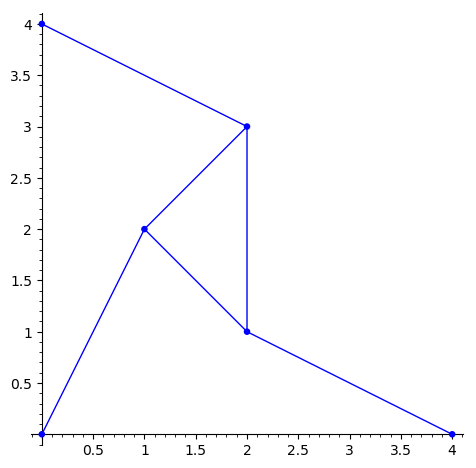
\includegraphics[scale=0.4]{lidur3aplot}
\end{center}
\columnbreak
\begin{center}
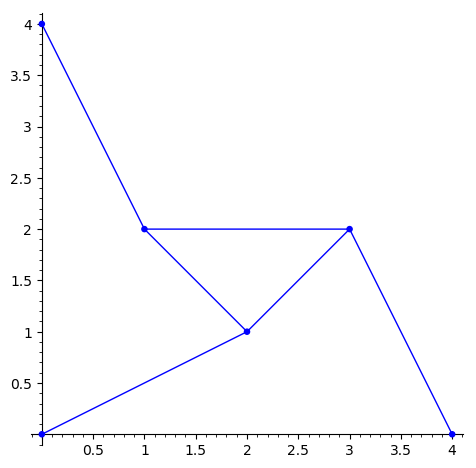
\includegraphics[scale=0.4]{lidur3bplot}
\end{center}
\end{multicols}

\vspace*{0.5cm}

Nú getum við næst teiknað graf $f$ með þessum nýju föstum (lið 4) með því að kalla á $g$ úr viðauka með eftirfarandi skipunum: \\

\begin{minted}{sage}
sage: h = g(5, 0, 6, 3, 3*sqrt(2), 3, pi/4, 5, 5, 3)
sage: plot(h, (-pi,pi))
\end{minted}

\vspace*{0.5cm}

sem gefur myndina: \\

\begin{center}
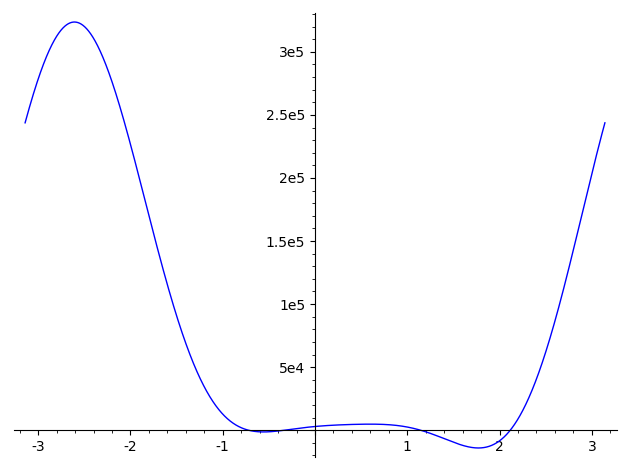
\includegraphics[scale=0.75]{lidur4aplot}
\end{center}

\vspace*{0.5cm}

Getum nú fundið allar núllstöðvarnar sem $f$ hefur með því að nýta okkur hjálparfallið \verb|find_all_roots| í viðauka ásamt hjálparfallinu \verb|xyfromth| til að finna $x$ og $y$ gildin sem samsvara lausnarhorninu $\theta$. Þetta getum við allt gert ásamt því að teikna samsvarandi myndir með eftirfarandi skipunum: \\

\begin{footnotesize}
\begin{minted}{sage}
sage: r = find_all_roots(g(5, 0, 6, 3, 3*sqrt(2), 3, pi/4, 5, 5, 3), -pi, pi)
sage: xys = [xyfromth(5, 0, 6, 3, 3*sqrt(2), 3, pi/4, 5, 5, 3, k) for k in r]
sage: for i in range(len(r)):
....:     plotter(5, 0, 6, 3, 3*sqrt(2), 3, xys[i][0], xys[i][1], r[i], pi/4)
\end{minted}
\end{footnotesize}

\vspace*{0.5cm}

Þá fáum við eftirfarandi fjórar myndir: \\

\begin{multicols}{2}
\begin{center}
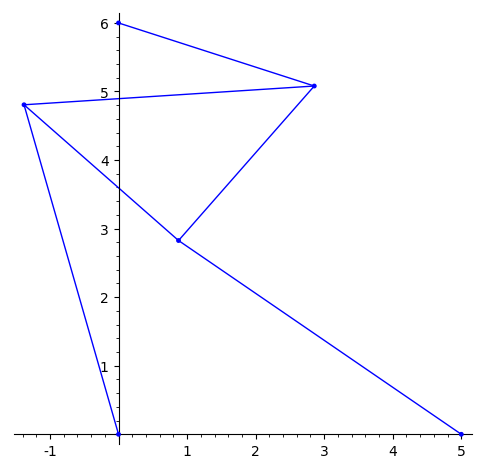
\includegraphics[scale=0.4]{lidur4b1plot}
\end{center}
\columnbreak
\begin{center}
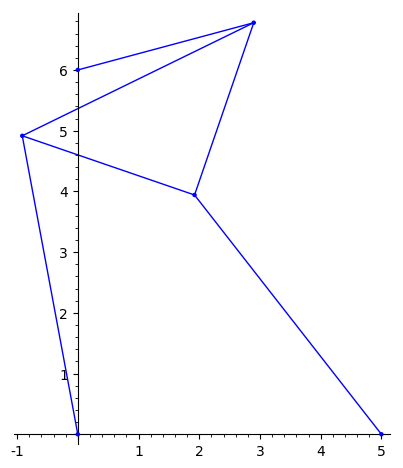
\includegraphics[scale=0.4]{lidur4b2plot}
\end{center}
\end{multicols}

\begin{multicols}{2}
\begin{center}
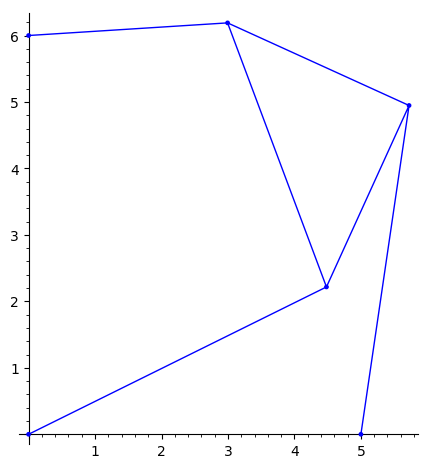
\includegraphics[scale=0.4]{lidur4b3plot}
\end{center}
\columnbreak
\begin{center}
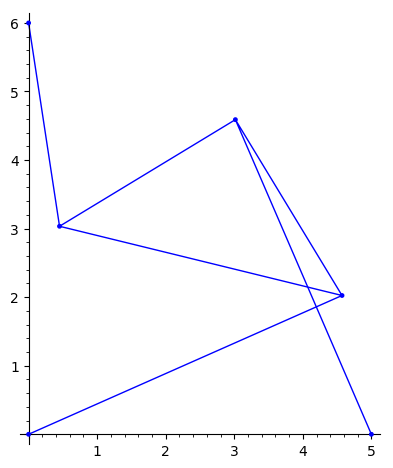
\includegraphics[scale=0.4]{lidur4b4plot}
\end{center}
\end{multicols}

\vspace*{0.5cm}

Auðvelt er að sjá útfrá myndunum að við fáum réttar lengdir á $p_1$,$p_2$ og $p_3$. Nú ef við breytum $p_2$ í $7$ getum við fengið sama plot nema fyrir þá breytingu með því að kalla á skipunina: \\

\begin{minted}{sage}
sage: h = g(5, 0, 6, 3, 3*sqrt(2), 3, pi/4, 5, 7, 3)
sage: plot(h, (-pi,pi))
\end{minted}

\vspace*{0.5cm}

Fáum þá eftirfarandi mynd: \\

\begin{center}
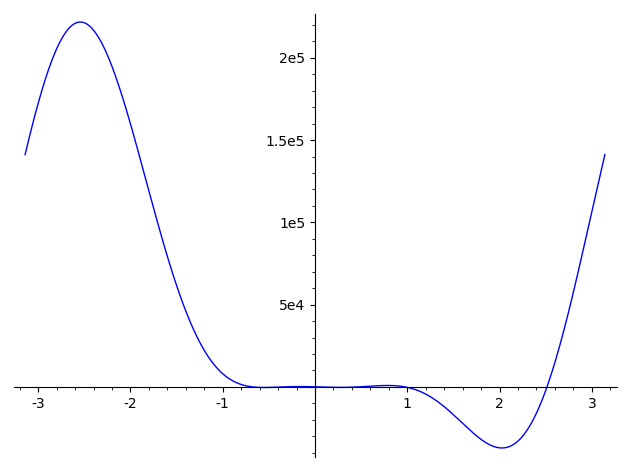
\includegraphics[scale=0.75]{lidur5aplot}
\end{center}

\vspace*{0.5cm}

Getum nú fundið allar núllstöðvar og samsvarandi myndir svipað og áður með skipununum: \\

\begin{footnotesize}
\begin{minted}{sage}
sage: r = find_all_roots(g(5, 0, 6, 3, 3*sqrt(2), 3, pi/4, 5, 7, 3), -pi, pi)
sage: xys = [xyfromth(5, 0, 6, 3, 3*sqrt(2), 3, pi/4, 5, 7, 3, k) for k in r]
sage: for i in range(len(r)):
....:     plotter(5, 0, 6, 3, 3*sqrt(2), 3, xys[i][0], xys[i][1], r[i], pi/4)
\end{minted}
\end{footnotesize}

\vspace*{0.5cm}

Þá fáum við eftirfarandi sex myndir: \\

\begin{multicols}{2}
\begin{center}
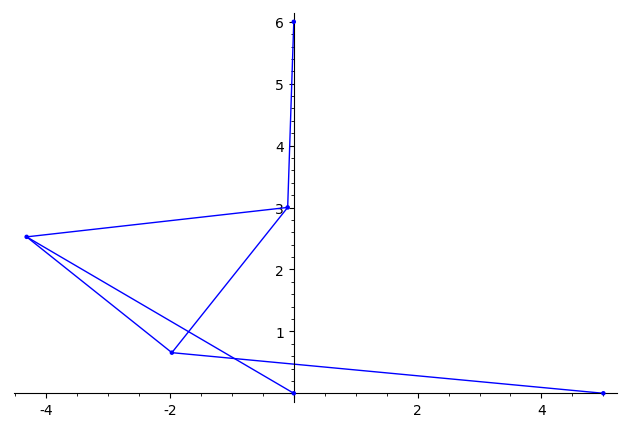
\includegraphics[scale=0.3]{lidur5b1plot}
\end{center}
\columnbreak
\begin{center}
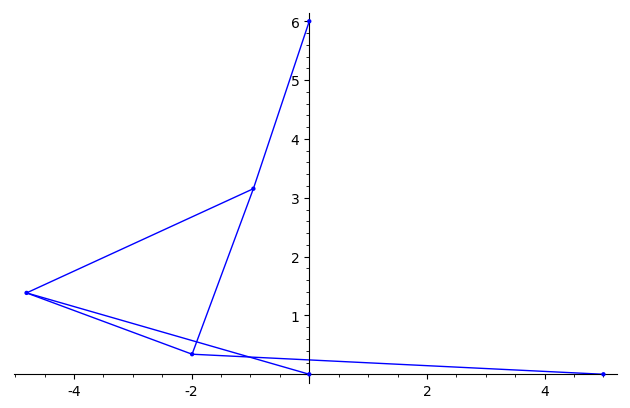
\includegraphics[scale=0.3]{lidur5b2plot}
\end{center}
\end{multicols}

\begin{multicols}{2}
\begin{center}
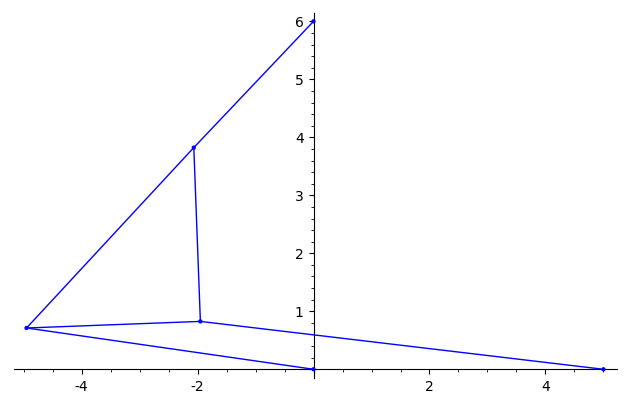
\includegraphics[scale=0.3]{lidur5b3plot}
\end{center}
\columnbreak
\begin{center}
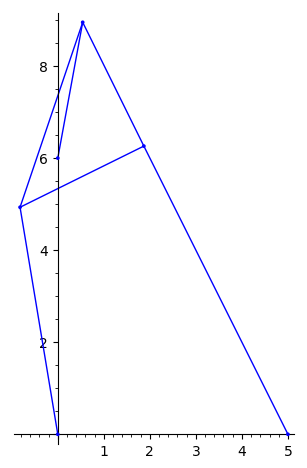
\includegraphics[scale=0.4]{lidur5b4plot}
\end{center}
\end{multicols}

\begin{multicols}{2}
\begin{center}
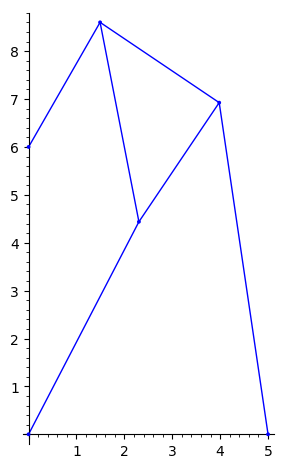
\includegraphics[scale=0.4]{lidur5b5plot}
\end{center}
\columnbreak
\begin{center}
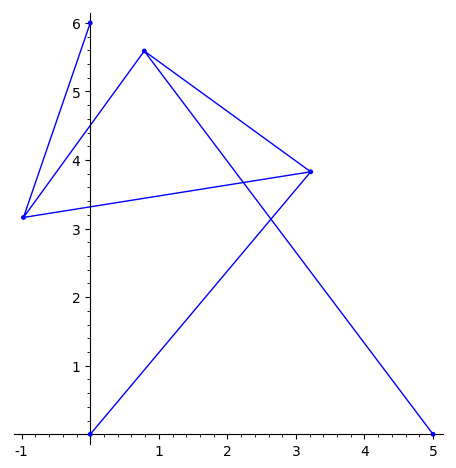
\includegraphics[scale=0.4]{lidur5b6plot}
\end{center}
\end{multicols}

\vspace*{0.5cm}

Við getum nú teiknað graf af fjölda lausna $f(\theta) = 0$ sem fall af $p_2$ með því að nýta hjálparfallið \verb|solsnumfromp2| og eftirfarandi skipun: \\

\begin{minted}{sage}
sage: h = solsnumfromp2(5, 0, 6, 3, 3*sqrt(2), 3, pi/4, 5, 3)
sage: plot(h, 0, 20)
\end{minted}

\vspace*{0.5cm}

Þetta gefur okkur eftirfarandi mynd: \\

\begin{center}
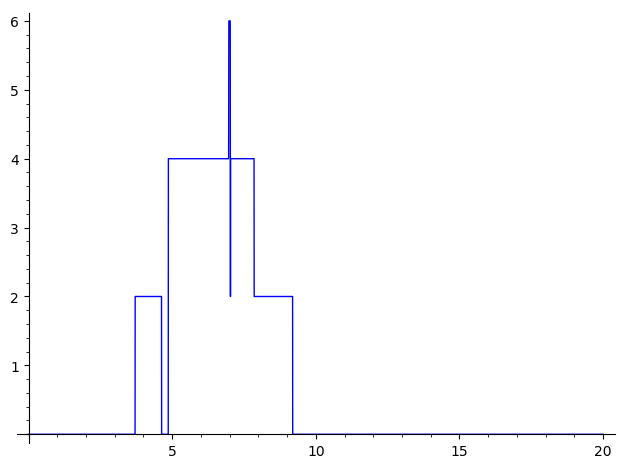
\includegraphics[scale=0.75]{lidur7plot}
\end{center}

\vspace*{0.5cm}

Þetta sýnir að ef við viljum hafa nákvæmlega tvær lausnir er m.a. hægt að velja $p_2 = 4$. Nú til að ákvarða nákvæma endapunkta hvers fallsgildisbils getum við notað eftirfarandi forritskóða: \\

\begin{minted}{sage}
sage: curh = solsnumfromp2(5, 0, 6, 3, 3*sqrt(2), 3, pi/4, 5, 3)
sage: curv = curh(0)
sage: changes = []
sage: for i in range(1000):
....:     nxtv = curh((i + 1) / 100)
....:     if nxtv != curv:
....:         changes.append((i / 100), (i + 1) / 100))
....:     curv = nxtv
\end{minted}

\vspace*{0.5cm}

Þetta gefur okkur 8 lítil bil sem skiptipunktarnir liggja í. Til þess að fá nákvæmari (upp að 9 aukastöfum) skiptipunkta notum við eftirfarandi forritskóða: \\

\begin{minted}{sage}
sage: exactchanges = [float("-inf")]
sage: for c in changes:
....:     lpos, rpos = c[0], c[1]
....:     lval, rval = curh(lpos), curh(rpos)
....:     while rpos - lpos > 1e-9:
....:         mpos = ((lpos + rpos) / 2).n()
....:         mval = curh(mpos)
....:         if mval == lval:
....:             lpos = mpos
....:         else:
....:             rpos = mpos
....:     exactchanges.append((lpos + rpos) / 2)
sage: exactchanges.append(float("inf"))
\end{minted}

\vspace*{0.5cm}

Nú loks til þess að fá hvaða fallgildi eru á hvaða bilum getum við loks notað eftirfarandi forritskóða: \\

\begin{minted}{sage}
sage: intervals = []
sage: for i in range(len(exactchanges) - 1):
....:     intervals.append(((exactchanges[i], exactchanges[i + 1]), 
....:         curh((exactchanges[i] + exactchanges[i + 1]) / 2)))
\end{minted}

\vspace*{0.5cm}

Þetta gefur okkur loks eftirfarandi niðurstöðu: \\

\begin{verbatim}
[((-inf, 3.71053114980459), 0),
 ((3.71053114980459, 4.63160214930773), 2),
 ((4.63160214930773, 4.86372385472059), 0),
 ((4.86372385472059, 6.96734398752451), 4),
 ((6.96734398752451, 7.02234040886164), 6),
 ((7.02234040886164, 7.03075937300920), 2),
 ((7.03075937300920, 7.84908692449331), 4),
 ((7.84908692449331, 9.19254726916552), 2),
((9.19254726916552, inf), 0)]
\end{verbatim}

\section*{Viðauki - kóði:}

\begin{minted}{sage}
def f(th):
    A2 = L3*cos(th)-x1
    B2 = L3*sin(th)
    A3 = L2*cos(th+gam) - x2
    B3 = L2*sin(th+gam) - y2
    D = 2*(A2*B3-B2*A3)
    if D == 0:
        raise ValueError("D is 0")
    N1 = B3*(p2**2-p1**2-A2**2-B2**2)
    N1 -= B2*(p3**2-p1**2-A3**2-B3**2)
    N2 = A2*(p3**2-p1**2-A3**2-B3**2)
    N2 -= A3*(p2**2-p1**2-A2**2-B2**2)
    return (N1**2+N2**2-p1**2*D**2).n()

def g(x1, x2, y2, L1, L2, L3, gam, p1, p2, p3):
    def f(th):
        A2 = L3*cos(th)-x1
        B2 = L3*sin(th)
        A3 = L2*cos(th+gam) - x2
        B3 = L2*sin(th+gam) - y2
        D = 2*(A2*B3-B2*A3)
        if D == 0:
            raise ValueError("D is 0")
        N1 = B3*(p2**2-p1**2-A2**2-B2**2)
        N1 -= B2*(p3**2-p1**2-A3**2-B3**2)
        N2 = A2*(p3**2-p1**2-A3**2-B3**2)
        N2 -= A3*(p2**2-p1**2-A2**2-B2**2)
        return (N1**2+N2**2-p1**2*D**2).n()
    return f

def plotter(x1, x2, y2, L1, L2, L3, x, y, th, gam):
    res = circle((0,0),0.025,fill=True,rgbcolor=(0,0,1))
    res += circle((x1,0),0.025,fill=True,rgbcolor=(0,0,1))
    res += circle((x2,y2),0.025,fill=True,rgbcolor=(0,0,1))
    res += circle((x,y),0.025,fill=True,rgbcolor=(0,0,1))
    res += circle((x+L3*cos(th),y+L3*sin(th)),
        0.025,fill=True,rgbcolor=(0,0,1))
    res += circle((x+L2*cos(th+gam),y+L2*sin(th+gam)),
        0.025,fill=True,rgbcolor=(0,0,1))
    res += line([(0,0),(x,y),(x+L2*cos(th+gam),
        y+L2*sin(th+gam))],rgbcolor=(0,0,1))
    res += line([(x1,0),(x+L3*cos(th),y+L3*sin(th)),
        (x,y)],rgbcolor=(0,0,1))
    res += line([(x2,y2),(x+L2*cos(th+gam),y+L2*sin(th+gam)),
        (x+L3*cos(th),y+L3*sin(th))],rgbcolor=(0,0,1))
    return res

def xyfromth(x1, x2, y2, L1, L2, L3, gam, p1, p2, p3, th):
    A2 = L3*cos(th)-x1
    B2 = L3*sin(th)
    A3 = L2*cos(th+gam) - x2
    B3 = L2*sin(th+gam) - y2
    D = 2*(A2*B3-B2*A3)
    if D == 0:
        raise ValueError("D is 0")
    N1 = B3*(p2**2-p1**2-A2**2-B2**2)
    N1 -= B2*(p3**2-p1**2-A3**2-B3**2)
    N2 = A2*(p3**2-p1**2-A3**2-B3**2)
    N2 -= A3*(p2**2-p1**2-A2**2-B2**2)
    return (N1/D).n(), (N2/D).n()

def find_all_roots(f, a, b, eps=0.0000000001):
    roots = []
    intervals_to_check = [(a,b)]
    while intervals_to_check:
        start, end = intervals_to_check.pop()
        try:
            root = find_root(f, start, end)
        except RuntimeError:
            continue
        if root in roots:
            continue
        if abs(f(root)) < 1:
            roots.append(root)
        intervals_to_check.extend([(start, root-eps), 
            (root+eps, end)])
    roots.sort()
    return roots

def solsnumfromp2(x1, x2, y2, L1, L2, L3, gam, p1, p3):
    def h(p2):
        def f(th):
            A2 = L3*cos(th)-x1
            B2 = L3*sin(th)
            A3 = L2*cos(th+gam) - x2
            B3 = L2*sin(th+gam) - y2
            D = 2*(A2*B3-B2*A3)
            if D == 0:
                raise ValueError("D is 0")
            N1 = B3*(p2**2-p1**2-A2**2-B2**2)
            N1 -= B2*(p3**2-p1**2-A3**2-B3**2)
            N2 = A2*(p3**2-p1**2-A3**2-B3**2)
            N2 -= A3*(p2**2-p1**2-A2**2-B2**2)
            return (N1**2+N2**2-p1**2*D**2).n()
        return len(find_all_roots(f, -pi, pi))
    return h
\end{minted}

\end{document}